\documentclass[
	a4paper,
	parskip
]{scrartcl}

\usepackage[english]{babel}
\usepackage{authblk}
\usepackage{amsthm}
\usepackage{amsmath}
\usepackage{amssymb}
\usepackage{booktabs}
\usepackage{float}
\usepackage{multirow}
\usepackage{physics}
\usepackage{siunitx}
\usepackage{hyperref}
\usepackage{cleveref}
\usepackage{subcaption}
\usepackage{pgfplots}
\usepackage[
  backend=biber,
  sorting=none
]{biblatex}
\usepackage[american]{circuitikz}
\usepackage{glossaries}
\usepackage[subpreambles=true]{standalone}

\addbibresource{literature.bib}

\makeglossaries
\newglossaryentry{s5990}{name=S5990, description={Hamamatsu two-dimensional PSD}}
\newacronym{psd}{PSD}{position-sensitive detector}
\newacronym{gbp}{GBP}{gain-bandwidth-product}

\title{Position-sensitive device}
\author{Bodo Kaiser}
\affil{Ludwig-Maximilians-Universität München}
\affil{\textit{bodo.kaiser@physik.uni-muenchen.de}}

\begin{document}

\maketitle
\tableofcontents

\section{Introduction}

We define a position-sensitive device as a device that outputs voltages proportional to the center of mass coordinates of a light beam incident on a sensitive area.

The present document summarizes the insights acquired on the journey of building such a device.

\subsection{Motivation}

Position-sensitive devices are used in a wide range of industrial and commercial applications, including displacement sensing and beam alignment, see Ref.~\cite[p.~22]{Maekynen00}.

We are interested in using a position-sensitive device for beam pointing alignment in our quantum optics laboratory.

The beam pointing refers to a laser beam's spatial focus and can change through thermal and mechanical effects.
Uncompensated changes in beam alignment can quickly degrade the overall performance of an optical system.
Therefore, it is crucial to align the beam pointing to ensure the optical system's proper operation at hand.

\subsection{Overview}

This document is organized as follows.

The first two sections introduce the theory of the (position-sensitive) photodiode and the operational amplifier.
These sections are rather elaborate and should be skipped by the pragmatic scientist.

The third section describes the (electrical) schematics of the detector.
If you want to adjust parameters, e.g., gain or bandwidth, you should read these sections.

The fourth section is the only significant section if you want to build a \gls{psd}.
If you also want an example of using the \gls{psd} in an optical setup to determine the spatial resolution, you should also read the fifth section.
Finally, the appendix gives some guidance on troubleshooting.

\subsection{Requirements}

The requirements are specified rather loose. The only hard requirement concerns the connectors and voltages of the power supply. The power connector should be a LEMO4 whose pin configuration is compatible with the \SI{\pm15}{\volt} dual-voltage power supplies used in the labs. Features that would be nice to have are:
\begin{enumerate}
	\item The device should be sensible with optical powers that are safe to operate, i.e., $P<\SI{1}{\micro\watt}$. There is no preferred wavelength.
	\item For easy integration into existing optical setups, the device should be as compact as possible. Additional space, if needed, should be occupied by elonging the height. The sensitive area of the detector should be on the bottom. The connectors should be on the top to avoid cables blocking the beam path.
	\item It should be possible to mount different detector sizes on the device.
\end{enumerate}
The range of the output voltages of the device can be chosen for the optimal signal-to-noise ratio.

\subsection{Specification}

\begin{figure}[H]
	\centering
	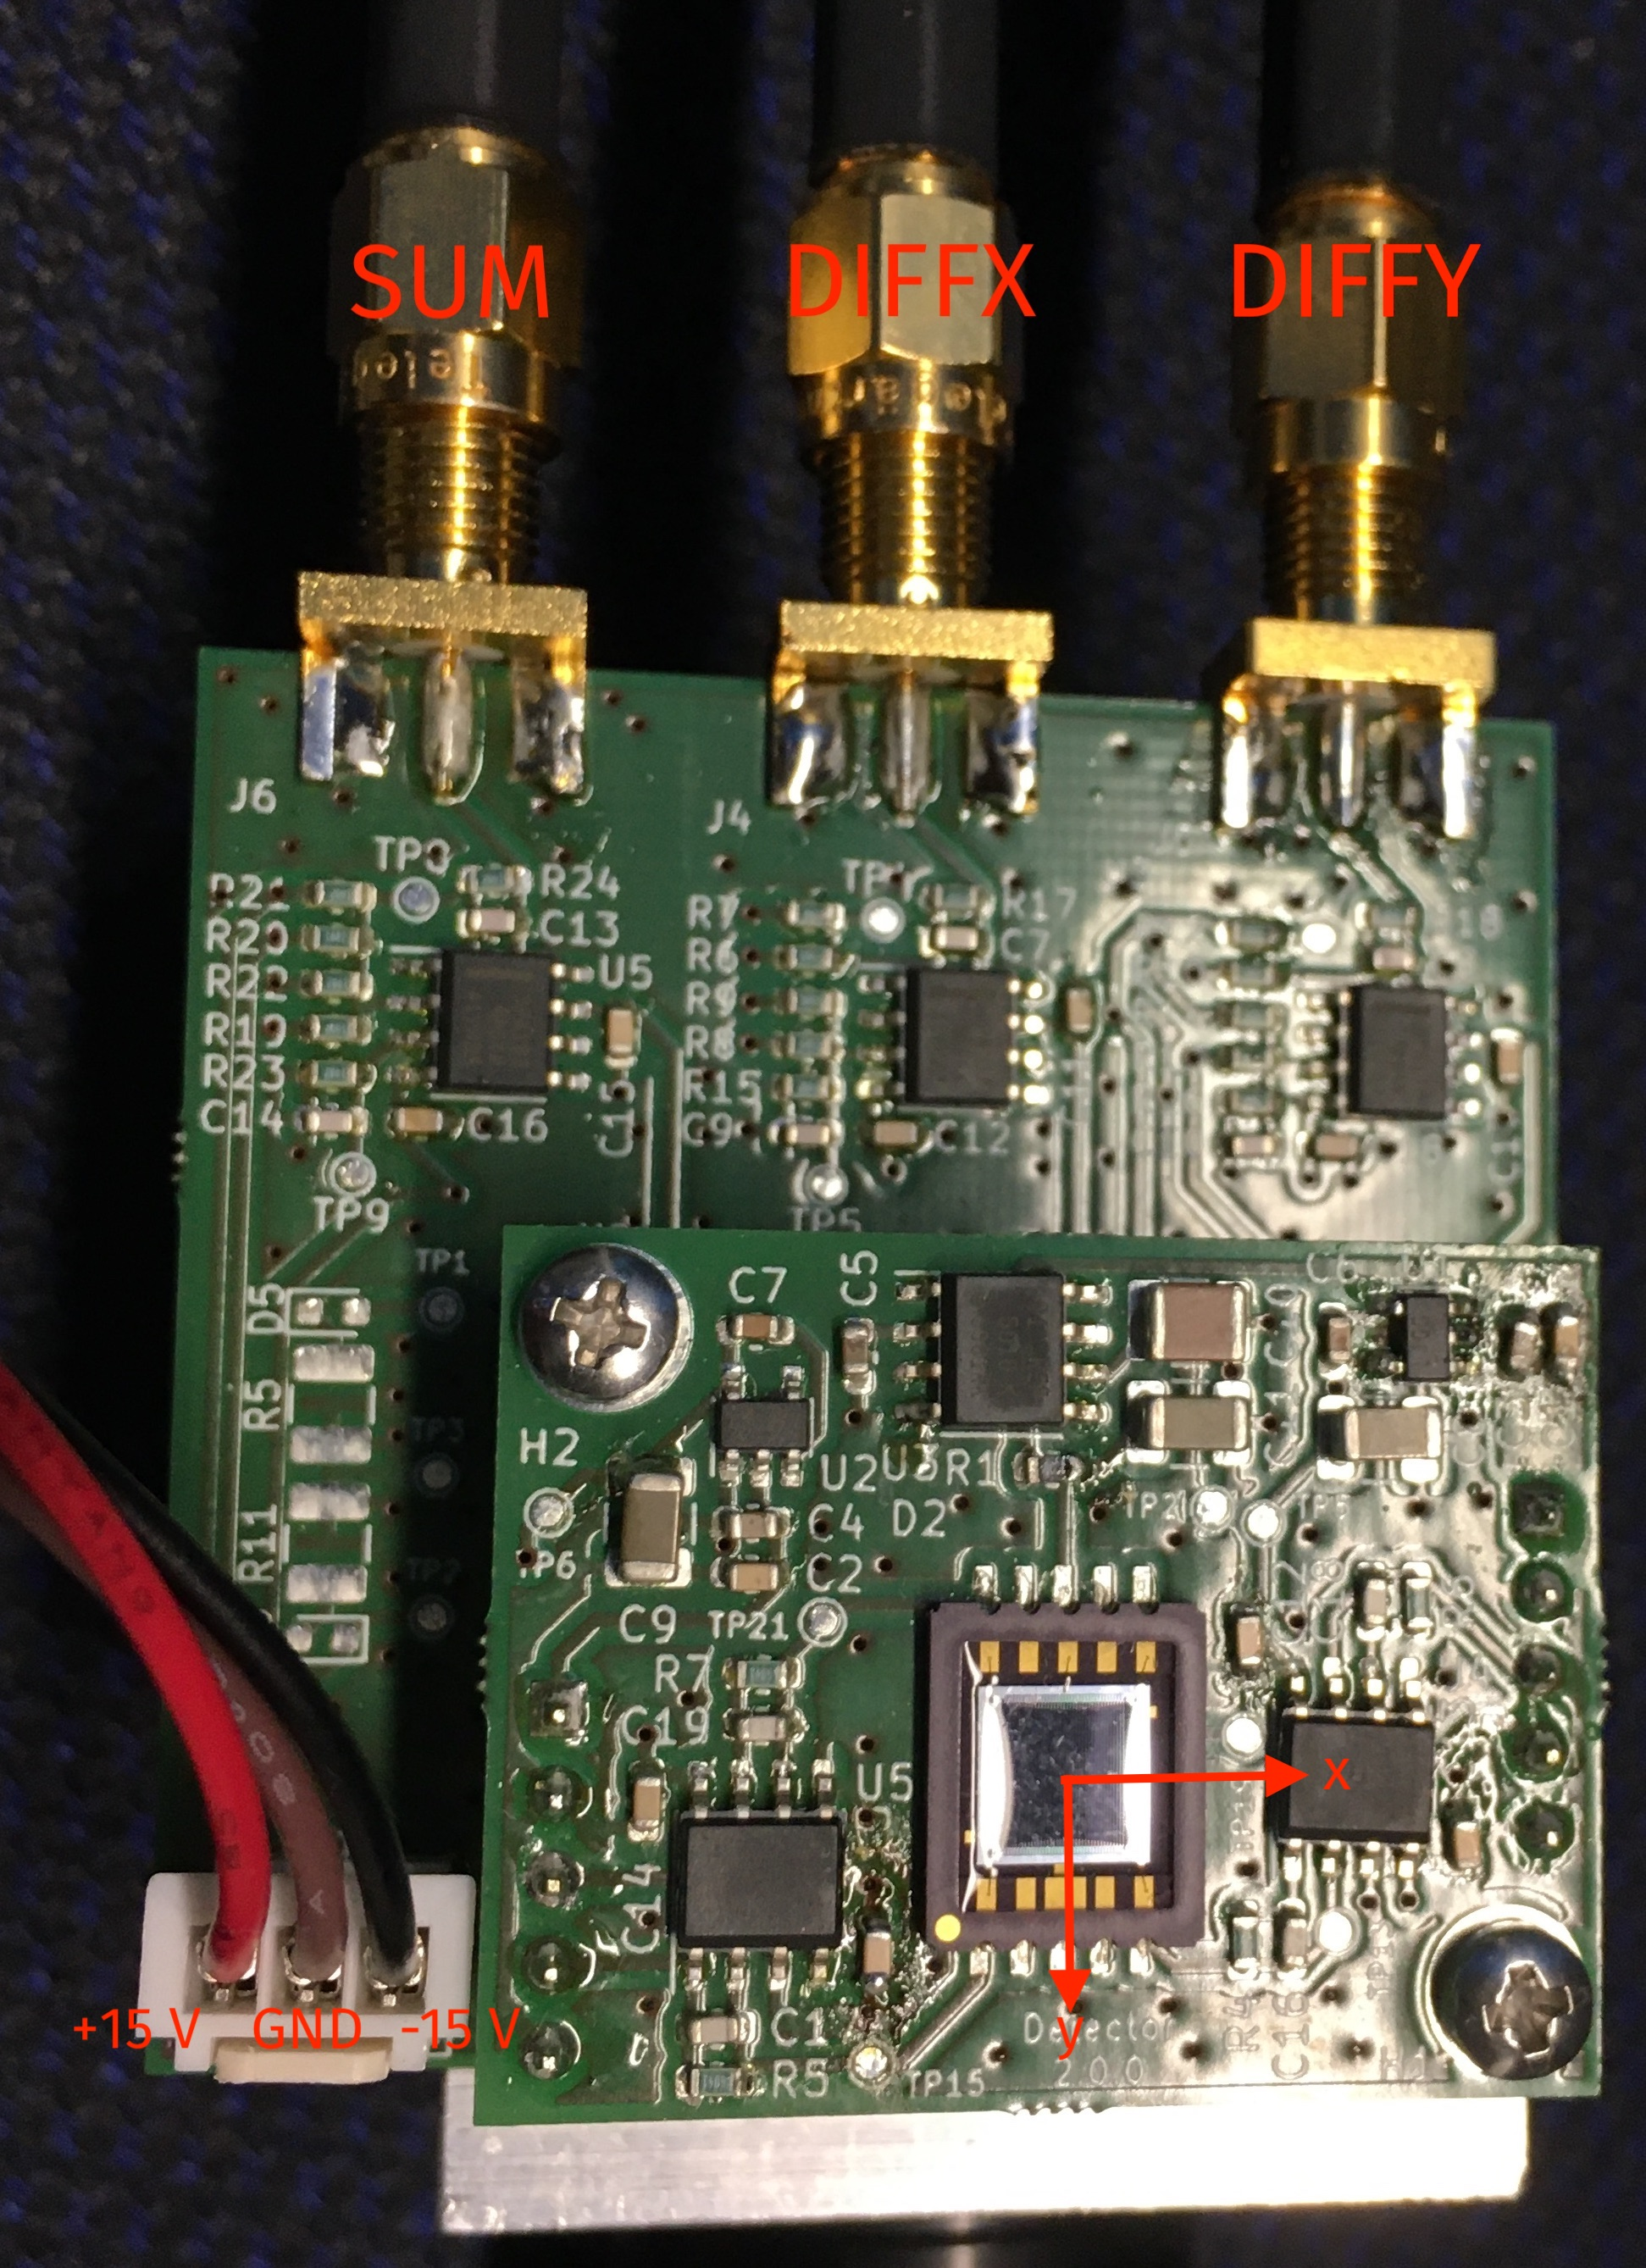
\includegraphics[scale=0.2]{detector.jpg}
	\caption{\gls{psd} on optical mount with connected cables}\label{fig:detector}
\end{figure}
\Cref{fig:detector} shows an image of the \gls{psd}.
The output voltage signals can be tapped from the upper \gls{sma} connectors.
The upper left connector gives the SUM voltage which reflects the total intensity of the optical signal.
The upper center connector gives the DIFFX voltage which reflects the difference proportional to the horizontal position on the sensitive area.
The upper right connector gives the DIFFY voltage which is proportional to the vertical position.
The SUM voltage is required to normalize the difference signals.
The DIFFX voltage increases when moving the light beam on the sensitive area to the right while the DIFFY voltage increases while moving the light beam to the bottom.
The device is powered by a 3-pin connector.
The outer (left) cable is the positive \SI{+15}{\volt} supply while the opposite cable is negative \SI{-15}{\volt} supply.
The center cable of the 3-pin connector has to reference ground.
The power connector has no polarity protection so be careful!

\begin{table}[htb]
  \centering
  \begin{tabular}{lcccc}
    \toprule
      Parameter & Minimum & Typical & Maximum \\
    \midrule
      Output voltages & \SI{-13}{\volt} & \SIrange{-2}{+2}{\volt} & \SI{+13}{\volt} \\
      Supply voltages & \SI{\pm13}{\volt} & \SI{\pm15}{\volt} & \SI{\pm37}{\volt} \\
      Spatial resolution & \SI{5.0}{\micro\meter} & \SI{2}{\micro\meter} & \SI{1}{\micro\meter} \\
      Bandwidth & & \SI{1400}{\kilo\hertz} & \\
    \bottomrule
  \end{tabular}
  \captionsetup{width=.8\textwidth}
  \caption{Specifications of the presented \gls{psd}}\label{tab:specifications}
\end{table}
\Cref{tab:specifications} summarizes the specifications of the presented \gls{psd}.
These specifications are only a rough estimate and we only assembled one \gls{psd} so far.
\section{Circuit theory}

\subsection{Transimpedance amplifier}

\subsection{Summing amplifier}
\section{Manufacturing}

% TODO: give rough description of manufacturing steps with images
\section{Electrical testing}
\section{Optical testing}

\printglossaries
\printbibliography

\end{document}